\documentclass[
  11pt,
  letterpaper,
   addpoints,
   answers
  ]{exam}

\usepackage{../exercise-preamble}
\usepackage{float}

\begin{document}
\pagestyle{headandfoot}
\firstpagefooter{ }{Página \thepage\ de \numpages}{ }
\runningfooter{ }{Página \thepage\ de \numpages}{ }

\noindent
\begin{minipage}{0.47\textwidth}

\includegraphics[width=\textwidth]{../fcfm_die.png}
\end{minipage}
\begin{minipage}{0.53\textwidth}
\begin{center} 
\large\textbf{Introducción a la Física Moderna} (F1100-5) \\
\large\textbf{Clase auxiliar 4} \\
\normalsize Prof.~ Rodrigo Soto.\\
\normalsize Prof.~Aux.~Erik Sáez - Javiera Toro 
\end{center}
\end{minipage}

\vspace{0.5cm}
\noindent
\vspace{.85cm}

\begin{questions}
%--------------------------
\question Un bloque de masa $m$ cuelga verticalmente de un resorte de constante elástica $k$ y largo natural $\ell_0$, y se mantiene en reposo en su posición de equilibrio. Considere el eje vertical positivo hacia abajo.
\begin{figure}[H]
  \centering
  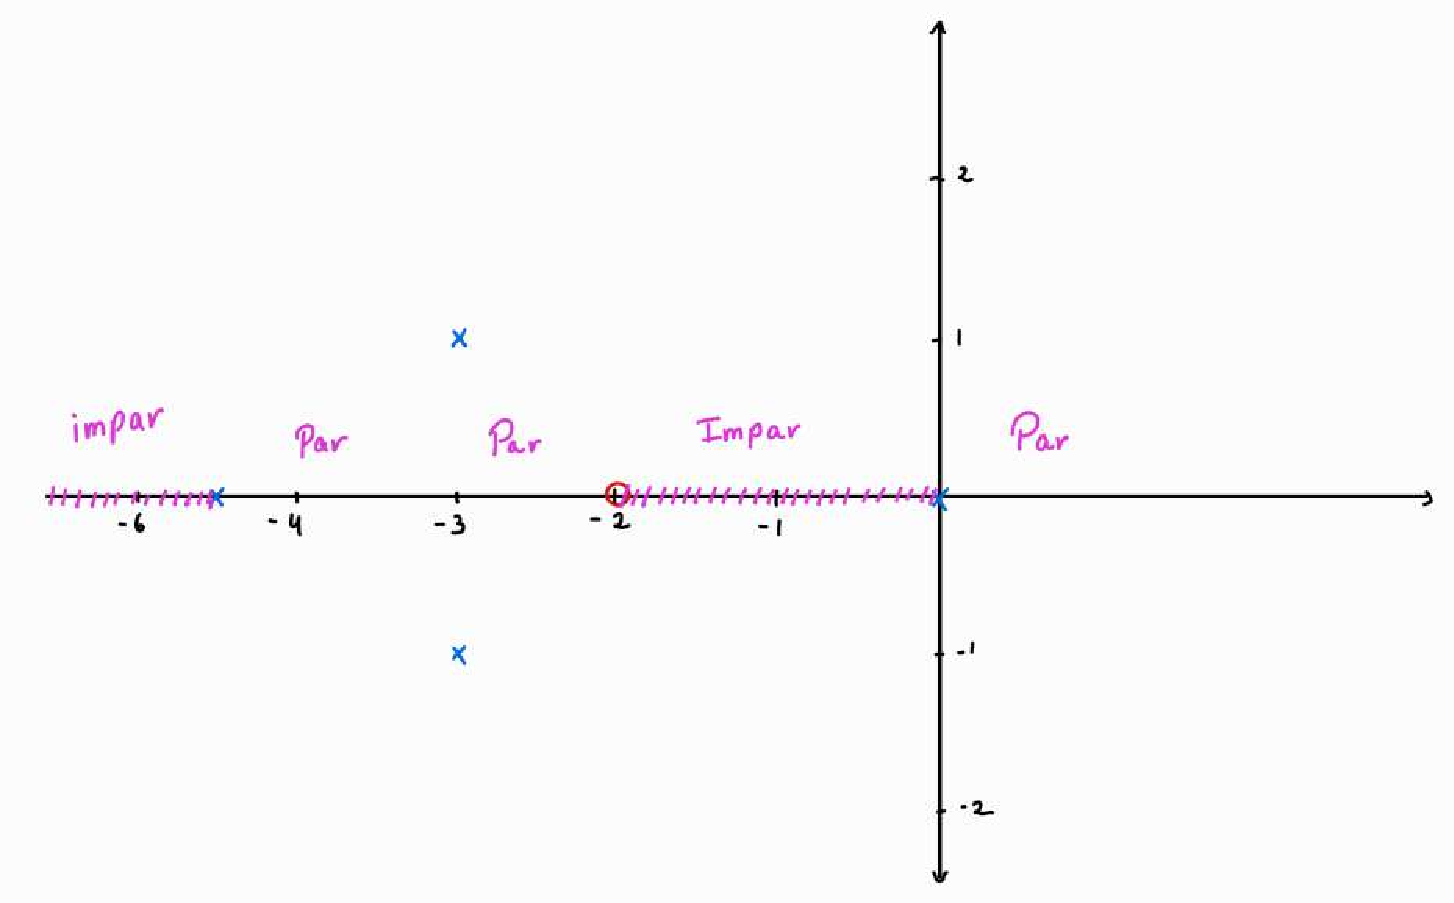
\includegraphics[width=0.6\textwidth]{Auxiliar_2_1}
  \caption{Bloque colgando de un resorte.}
  \label{fig:spring_block}
\end{figure}
\begin{parts}
  \part Encuentre la posición de equilibrio del bloque.
  \part De pronto, el techo que sostiene al resorte comienza a oscilar como $y_t(t)=A\cos(\Omega t)$. Encuentre la ecuación de movimiento del bloque.
  \part Calcule la amplitud del movimiento.
\end{parts}
%--------------------------
\begin{solution}
  \subsection*{Resolución 1.1}
  Usaremos el eje vertical positivo hacia abajo. Sea $y(t)$ la posición del bloque medida desde un origen y $y_t(t)$ la posición del punto de suspensión (techo). La elongación del resorte es $\,(y-y_t)-\ell_0$. Aplicamos la segunda ley de Newton al bloque (en equilibrio el techo está fijo, $y_t=0$):
  \begin{equation}
    m\ddot{y} = mg - F_e, 
    \qquad F_e = k\,(y - \ell_0),
  \end{equation}
  donde $F_e$ es el módulo de la fuerza elástica (dirigida hacia arriba). Sustituyendo:
  \begin{align}
    m\ddot{y} &= mg - k(y - \ell_0), \\
    \ddot{y} &= -\frac{k}{m}(y - \ell_0) + g, \\
    \ddot{y} &= -\frac{k}{m}\left(y - \ell_0 - \frac{mg}{k}\right).
  \end{align}
Realizamos el cambio de variables conveniente:
  \begin{align}
    z &= y - \ell_0 - \frac{mg}{k}, \\
    \ddot{z} &= \ddot{y},
  \end{align}
  con lo que la ecuación se convierte en
  \begin{equation}
    \ddot{z} = -\frac{k}{m}z,
  \end{equation}
  El movimiento corresponde a un movimiento armónico simple con frecuencia natural $\omega^2 = \tfrac{k}{m}$. La posición de equilibrio se obtiene imponiendo $\ddot{z}=0 \;\Rightarrow\; z=0$,
  es decir
  \begin{equation}
    y_0 = \ell_0 + \frac{mg}{k}.
  \end{equation}
Por lo tanto, la posición de equilibrio del bloque está desplazada una distancia $\tfrac{mg}{k}$ respecto de la longitud natural del resorte.

  \subsection*{Resolución 1.2}

Si dibujamos el sistema en algún tiempo arbitrario, tenemos el siguiente esquema:
\begin{figure}[H]
  \centering
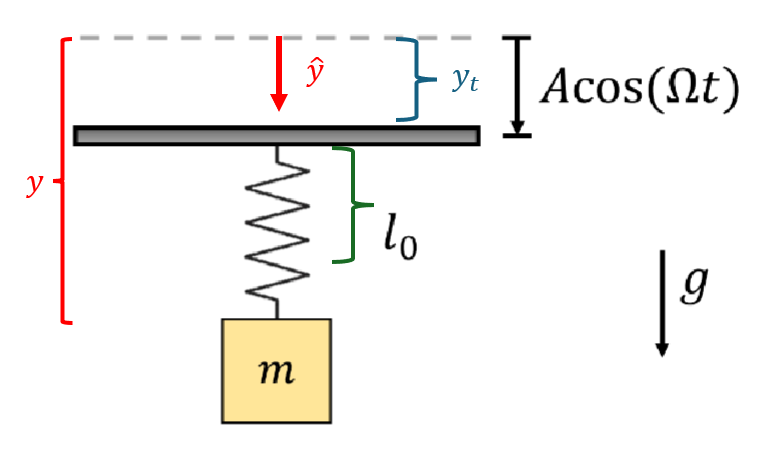
\includegraphics[width=0.6\textwidth]{Auxiliar_2_4}
  \caption{Bloque colgando de un resorte.}
  \label{fig:spring_block}
\end{figure}

Se observa que lo único que cambiará en el DCL es la fuerza elástica, que ahora depende de la posición del techo $y_t(t)$, por lo tanto tenemos que:
  \begin{equation}
    F_e = k\big[y - \ell_0 - y_t(t)\big].
  \end{equation}

  Aplicando la segunda ley de Newton al bloque:
  \begin{align}
    m\ddot{y} = mg - k\big[y - \ell_0 - y_t(t)\big], \\
    \ddot{y} + \frac{k}{m}\left(y - \ell_0 - \frac{mg}{k}\right) = \frac{k}{m}y_t(t).
  \end{align}

  Introduciendo el cambio de variable
  \begin{equation}
    z = y - \ell_0 - \frac{mg}{k},
    \qquad \ddot{z} = \ddot{y},
  \end{equation}
  resulta
  \begin{equation}\label{eq_mov}
    \ddot{z} + \omega^2 z = \omega^2 A \cos(\Omega t),
    \qquad \omega^2 = \frac{k}{m}.
  \end{equation}

Esta es la ecuación de movimiento del bloque: un oscilador armónico forzado (sin amortiguamiento). Donde las soluciones serán de la forma
\begin{equation*}
  z(t)=C_1\cos(\omega t)+C_2\sin(\omega t)
       +\frac{\omega^2 A}{\omega^2-\Omega^2}\cos(\Omega t),\qquad (\Omega\ne\omega).
\end{equation*}
En resonancia ($\Omega=\omega$), la solución particular crece linealmente en el tiempo:
\begin{equation*}
  z_p(t)=\frac{A\,\omega}{2}\,t\,\sin(\omega t).
\end{equation*}
Finalmente, la coordenada original es $y(t)=z(t)+\ell_0+\tfrac{mg}{k}$.

  \subsection*{Resolución 1.3}

De la ecuación \eqref{eq_mov} reconocemos la forma estándar del oscilador
  forzado:
  \begin{equation}
    \ddot{z} + \omega^2 z = \frac{F_0}{m}\cos(\Omega t),
    \qquad \frac{F_0}{m} = \omega^2 A.
  \end{equation}

  Por lo tanto, la amplitud de la respuesta estacionaria es
  \begin{equation}
    B = \frac{F_0/m}{\omega^2 - \Omega^2}
      = \frac{\omega^2 A}{\omega^2 - \Omega^2}.
  \end{equation}
  Nótese que, en ausencia de amortiguamiento, la amplitud crece sin cota cuando $\Omega \to \omega$ (resonancia).
\end{solution}
%--------------------------
\question Una cuerda está dispuesta horizontalmente entre dos puntos separados por una distancia $L$. Tiene densidad lineal $\rho$ y está sometida a una tensión $T$. Ambos extremos de la cuerda se hacen oscilar con una aceleración vertical de la forma $a_0\sin(\Omega t)$.

Se desea determinar la forma $y(x,t)$ de las ondas estacionarias formadas en la cuerda. Para esto, considere como solución la superposición de ondas sinusoidales que viajan en direcciones opuestas:
\[
  y(x,t) = A\sin(kx-\omega t) + B\sin(kx+\omega t).
\]

\begin{parts}
  \part Escriba las condiciones de borde en los puntos $x=0$ y $x=L$.
  \part Imponga estas condiciones de borde y encuentre las relaciones entre: $\Omega$ y $\omega$; $a_0$, $A$, $B$ y $\Omega$; y entre $A$ y $B$. Además escriba la función de onda $y(x,t)$.
  \part Compare con la solución para ambos extremos fijos y comente.
\end{parts}

  	\textit{Indicación: puede ser útil la relación trigonométrica}
\[
  \sin(\phi) \pm \sin(\theta) = 2\,\sin\!\left(\frac{\phi \pm \theta}{2}\right)\,\sin\!\left(\frac{\phi \mp \theta}{2}\right).
\]
%--------------------------
\begin{solution}
  \subsection*{Resolución 2.1}
  Tenemos una onda estacionaria forzada en donde los extremos se mueven con una aceleracion dada y las condiciones de borde que se deben cumplir son:
  \begin{align}
    \ddot y(0,t)&=a_0\sin(\Omega t) \\
    \ddot y(L,t)&=a_0\sin(\Omega t).
  \end{align}

  \subsection*{Resolución 2.2}
  Se busca imponer las condiciones de borde, por lo tanto tendremos primeramente que:
  \begin{align}
    y(x,t)&=A\sin(kx-\omega t)+B\sin(kx+\omega t)\\
    \dot{y}(x,t)&=\omega\big[A\cos(kx-\omega t)-B\cos(kx+\omega t)\big].\\
    \ddot{y}(x,t)&=-\omega^2\big[A\sin(kx-\omega t)+B\sin(kx+\omega t)\big].
  \end{align}
Luego al imponer las condiciones de borde se logra obtener que:
\begin{align}
  \ddot{y}(x =0,t)&= -\omega^{2}A\sin(-\omega t) - \omega^{2}B\sin(\omega t)  = a_{0}\sin(\Omega t)
\end{align}
Recordemos que la funcion $\sin$ cumple con $\sin(-\theta)=-\sin(\theta)$, por lo que:
\begin{align}
  \ddot{y}(x=0,t) = A\omega^{2}\sin(\omega t) - B\omega^{2}\sin(\omega t) = \omega^{2}(A-B)\sin(\omega t) = a_{0}\sin(\Omega t)
\end{align}
La única forma de que esto sea válido es que para todo $t$ se cumpla que:
  \begin{equation}
    \boxed{
    \Omega=\omega,\qquad A-B=\frac{a_0}{\omega^2}
  }
  \end{equation}
  Por otro lado podemos evaluar la otra condición de borde en $x=L$ con lo que se tendra:
  \begin{align}
    \ddot{y}(x = L,t)&= -\omega^{2}A\sin(kL-\omega t) - \omega^{2}B\sin(kL+\omega t) = a_{0}\sin(\Omega t)
  \end{align}
  En relación a las condiciones anteriores derivamos que $(A-B)\omega^{2} = a_{0}$ y que $\omega= \Omega$ por lo tanto al reemplazar tendremos que:
  \begin{align}
    -A\sin(kL-\omega t) - B\sin(kL+\omega t) &= (a-B)\sin(\omega t).\\
    -A\sin(kL-\omega t) - A\sin(\omega t) &= \sin(kL+\omega t) - B\sin(\omega t).
  \end{align}
  Ahora usaremos las identidades trigonometricas dadas por:
  \begin{align}
    \sin(\phi) \pm \sin(\theta) = 2\,\sin\!\left(\frac{\phi \pm \theta}{2}\right)\,\sin\!\left(\frac{\phi \mp \theta}{2}\right).
  \end{align}
  Que para nuestro caso particular viene dada por:
  \begin{align}
    -A\left(2\sin\left(\frac{kL-\omega t+\omega t}{2}\right)\cos\left(\frac{kL-\omega t-\omega t}{2}\right)\right) &= B\left(2\cos\left(\frac{kL+\omega t+\omega t}{2}\right)\sin\left(\frac{kL+\omega t-\omega t}{2}\right)\right) \\
    -A\sin\left(\frac{kL}{2}\right)\cos\left(\frac{kL}{2} - \omega t\right) &= B\sin\left(\frac{kL}{2}\right)\cos\left(\frac{kL}{2} + \omega t\right)
  \end{align}
  Es importante notar que esto se debe cumplir para todo tiempo, en particular para $t=0$, por lo tanto:
  \begin{align}
    -A\cos\left(\frac{kL}{2}\right) &= B\cos\left(\frac{kL}{2}\right)\\
    -A &= B
  \end{align}
  Con lo que en base a lo obtenido con la condicion anterior se deriva finalmente que $2A = \frac{a_{0}}{\omega^2}$. Con lo que la solucion finalmente vendra dada por:
\begin{align}
  y(x,t) &= Asin(kx - \omega t) + Bsin(kx + \omega t)\\
  &= A\left(\sin(kx - \omega t) - \sin(kx + \omega t)\right)\\
  &= 2A\sin(-\omega t )\cos(kx)\\
  &= - \frac{2a_{0}}{\omega^2}\sin(\omega t)\cos(kx)
\end{align}
  \subsection*{Resolución 2.3}
  Con ambos extremos fijos se exige $y(0,t)=y(L,t)=0$, lo que da $k=n\pi/L$ para todo entero $n$. Aquí, en cambio, las CB prescriben la \emph{aceleración} de los extremos, seleccionando solo los modos con $kL=2\pi n$ (equivalentes a los $n$ pares del caso de extremos fijos). Además, los extremos no son nodos: se mueven en fase con $\ddot y(0,t)=\ddot y(L,t)=a_0\sin(\omega t)$.
\end{solution}
%--------------------------
\question  Considere una cuerda de masa $M$ y longitud $L$, sometida a una tensión $T$ con ambos extremos fijos. Mediante un mecanismo electromecánico se hace oscilar el punto medio $\big(L/2\big)$ con una velocidad
\begin{equation}
  v(t)=v_0\sin(\Omega t).
\end{equation}

\begin{figure}[h!]
\centering
\begin{tikzpicture}[
  x=1.35cm, y=1.35cm, line cap=round, >=Latex,
  every node/.style={scale=1.02}
]
  % ---- Parámetros ----
  \def\L{10}           % distancia entre caras internas de los soportes
  \def\W{0.70}         % ancho de los soportes (más grandes)
  \def\yTop{1.10}      % cota de la barra superior
  \def\yBot{0.00}      % cota de la barra inferior
  \def\mid{\L/2}       % punto medio

  % ---- Soportes hachurados (más altos y anchos) ----
  \fill[pattern=north east lines, pattern color=gray!70, draw=gray!60]
       (-\W,\yTop+0.25) rectangle (0,\yBot-0.25);
  \fill[pattern=north east lines, pattern color=gray!70, draw=gray!60]
       (\L,\yTop+0.25) rectangle (\L+\W,\yBot-0.25);

  % ---- Barra superior (solo hasta la mitad, para L/2) ----
  \draw[thick] (0,\yTop) -- (\mid,\yTop);

  % ---- Barra inferior (completa, para L) ----
  \draw[thick] (0,\yBot) -- (\L,\yBot);

  % ---- Cuerda (curva roja, extremos fijos) ----
  \draw[very thick, red]
    (0,0.06) .. controls (\mid*0.60,0.7) and (\mid*1.40,0.7) .. (\L,0.06);

  % ---- Centro: línea discontinua + flecha doble del forzamiento ----
  \draw[densely dashed] (\mid,0.12) -- (\mid,0.98);
  \draw[-{Latex[length=2mm]}] (\mid,0.55) -- ++(0,0.33);   % flecha hacia arriba
  \draw[-{Latex[length=2mm]}] (\mid,0.55) -- ++(0,-0.33);  % flecha hacia abajo
  \node[anchor=west] at (\mid+0.15,0.7) {$v_0\sin(\Omega t)$};

  % ---- Flecha de dos puntas para L/2 (arriba) ----
  \draw[<->] (0,\yTop+0.20) -- (\mid,\yTop+0.20);
  \node at (\mid/2,\yTop+0.8) {$\displaystyle \frac{L}{2}$};

  % ---- Flecha de dos puntas para L (abajo) ----
  \draw[<->] (0,\yBot-0.20) -- (\L,\yBot-0.20);
  \node at (\L/2,\yBot-0.4) {$\displaystyle L$};
\end{tikzpicture}
\caption{Forzamiento en el punto medio con extremos fijos.}
\end{figure}



\begin{parts}
  \part Escriba las condiciones de borde apropiadas para el sistema.
  \part Suponiendo soluciones de la forma
    \begin{equation}
      y(x,t) = A\sin(kx-\omega t) + B\sin(kx+\omega t),
    \end{equation}
    encuentre las longitudes de onda de los modos de oscilación.
  \part Bosqueje los primeros 3 modos.
  \part Escriba la función $y_n(x,t)$, simplificada en función del forzamiento $v(t)$,
    para la forma de la onda en el $n$-ésimo modo.
\end{parts}
%--------------------------
\begin{solution}
\subsection*{Resolución 3.1}
Extremos fijos y forzamiento de velocidad en el punto medio:
\begin{align}
  y(0,t) &= 0, &
  y(L,t) &= 0, &
  \left.\frac{\partial y}{\partial t}\right|_{x=L/2} &= v_0\,\sin(\Omega t).
\end{align}

\subsection*{Resolución 3.2}
Suponiendo soluciones de la forma
\begin{align}
  y(x=0,t)&=A\sin(-\omega t)+B\sin(\omega t)= 0\\
          -A\sin(\omega t)&= -B\sin(\omega t)\\
          A &= B
\end{align}
Dado que tenemos que $A=B$, luego tenemos,
\begin{align}
  y(x,t)&= A\left(\sin(kx - \omega t) + \sin(kx + \omega t)\right)\\
  y(x,t)&= 2A\sin(kx)\cos(\omega t)
\end{align}
Para lo cual utilizamos la identidad de ángulo suma para senos y cosenos:
\begin{align}
  \sin(\alpha) + \sin(\beta) &= 2\sin\left(\frac{\alpha + \beta}{2}\right)\cos\left(\frac{\alpha - \beta}{2}\right)
\end{align}
Luego, para la otra condición en $x=L$, se obtiene
\begin{align}
  y(x=L,t)&=2A\sin(kL)\cos(\omega t)=0\\
  \sin(kL)&=0 \quad \cos(\omega t)\ne 0\\
  kL &= n\pi, \quad n=1,2,3,\dots
\end{align}
De aquí,
\begin{align}
  k= \frac{2\pi}{\lambda} \quad \Rightarrow \quad kL=n\pi = \frac{2\pi L}{\lambda}
\end{align}
Con lo que $\boxed{\lambda_n = \tfrac{2L}{n}}$. Además,
\begin{align}
  y(x,t) &= 2A\sin(kx)\cos(\omega t),\\
  \dot{y}(x,t) &= -2A\,\omega\,\sin(kx)\,\sin(\omega t).
\end{align}
Imponiendo la condición de borde de velocidad en el punto medio,
\begin{align}
  \left.\dot{y}\,\right|_{x = L/2} &= -2A\omega \,\sin\!\left(\frac{n \pi}{2}\right)\sin(\omega t) \;=\; v_0 \,\sin(\Omega t).
\end{align}
Por lo tanto, debe cumplirse para todo $t$ que
\begin{align}
  \Omega = \omega,\qquad v_{0} = -2A\omega \,\sin\!\left(\frac{n\pi}{2}\right).
\end{align}
Si $n$ es par, $\sin(n\pi/2)=0$ y entonces $v_0=0$ (no se puede imponer la velocidad): \textbf{solo se excitan los modos impares}. En consecuencia,
\begin{align}
  n=1,3,5,\dots,\qquad \lambda_n = \frac{2L}{n}.
\end{align}

\subsection*{Resolución 3.3}
Para los primeros 3 modos excitados ($n=1,3,5$) tenemos gráficamente:
\begin{figure}[H]
  \centering
  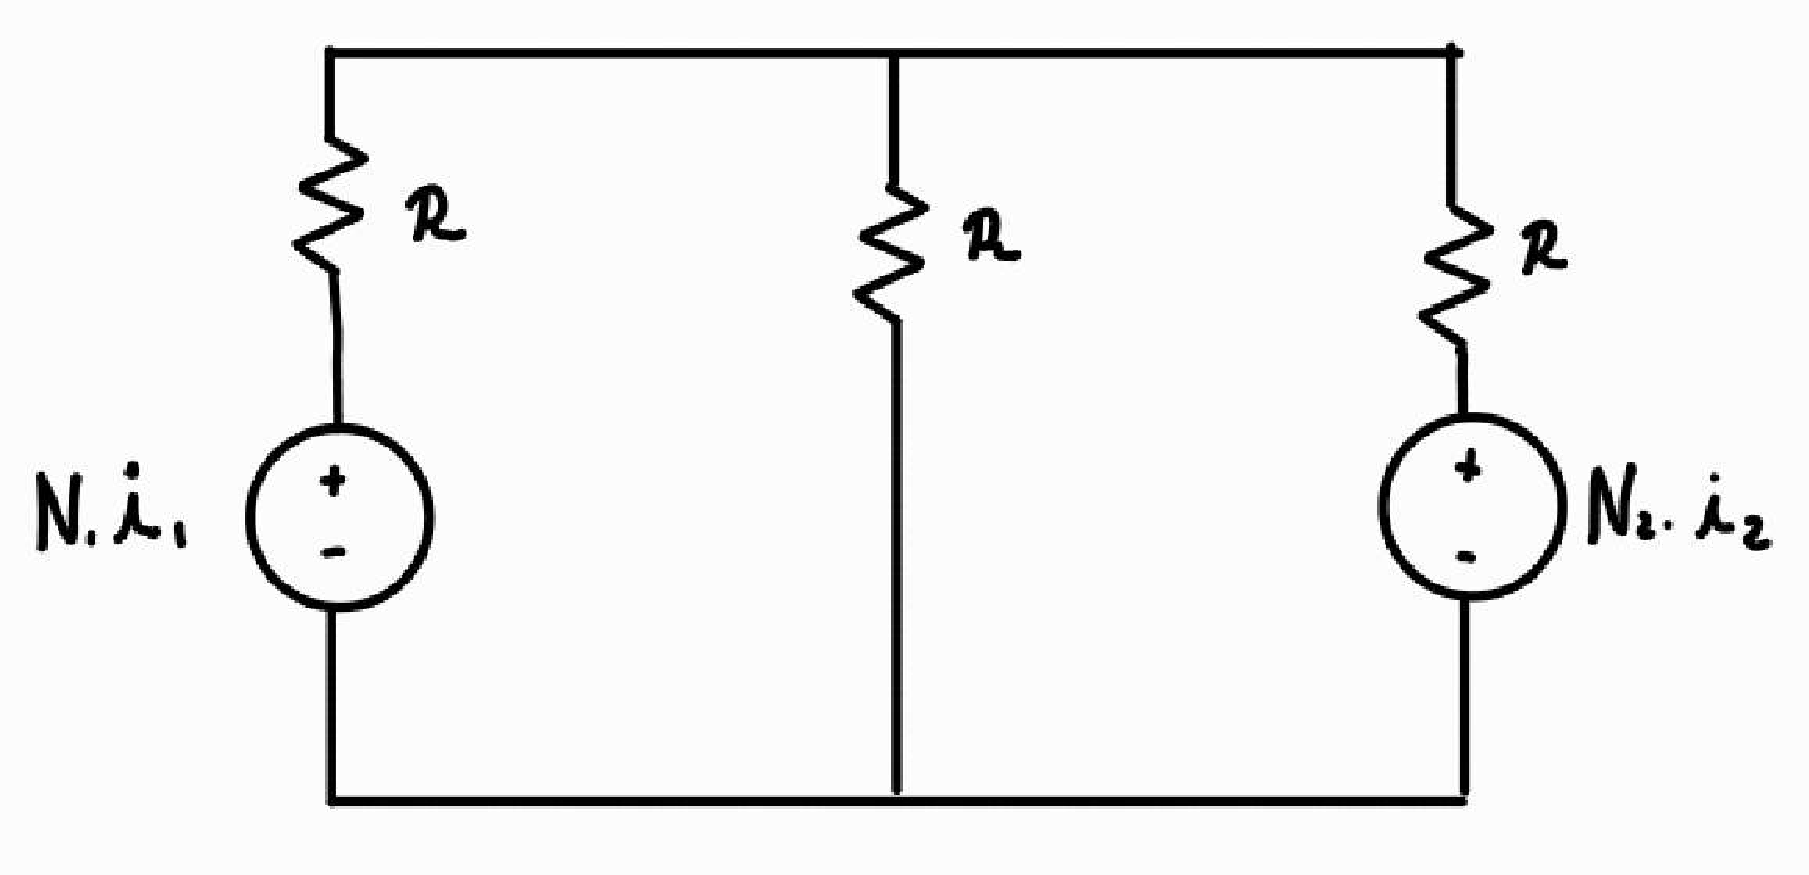
\includegraphics[width=.5\linewidth]{Auxiliar_2_2}
  \caption{Formas espaciales normalizadas de los primeros tres modos excitados (impares).}
  \label{fig:modos}
\end{figure}
\subsection*{Resolución 3.4}
Por último, de la condición en el centro se obtiene, para $n$ impar,
\begin{align}
  A = -\frac{v_0}{2\Omega\,\sin(n\pi/2)} \;=\; -\frac{v_0}{2\Omega}\,(-1)^{\frac{n-1}{2}}.
\end{align}
Por lo tanto, usando $k_n=\tfrac{n\pi}{L}$, la forma del $n$-ésimo modo (impar) es
\begin{align}
  y_n(x,t) 
  &= 2A\,\sin\!\left(\frac{n\pi}{L}x\right)\cos(\Omega t)\\
  &= -\,\frac{v_0}{\Omega}\,(-1)^{\frac{n-1}{2}}\,\sin\!\left(\frac{n\pi}{L}x\right)\cos(\Omega t),\qquad n=1,3,5,\dots
\end{align}
equivalentemente, $(-1)^{\frac{n-1}{2}}=\operatorname{sgn}[\sin(n\pi/2)]$.
\end{solution}
%--------------------------
\question Considere una cuerda de densidad lineal $\rho$ y largo $L$ que se cuelga del techo
sin sostener ninguna masa, como se indica en la figura. Se golpea la cuerda en el
centro generando dos pulsos que se propagan, uno ascendente y otro descendente.
\begin{figure}[H]
  \centering
  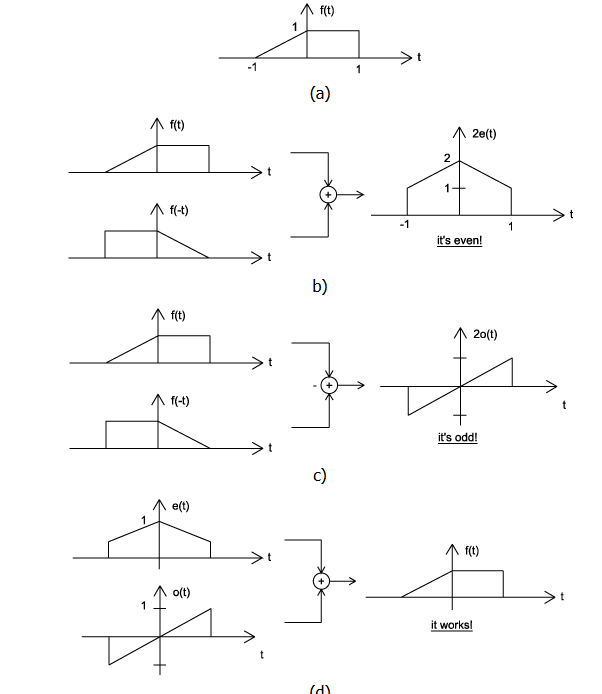
\includegraphics[width=0.35\textwidth]{Auxiliar_2_3}
  \caption{Cuerda colgante golpeada en el centro: pulsos ascendente y descendente.}
  \label{fig:cuerda-colgante}
\end{figure}

\begin{enumerate}
  \item ¿Cuál de los pulsos llegará primero al extremo correspondiente de la cuerda?
  \item Al llegar al respectivo borde, cada pulso será reflejado. Diga si los pulsos se reencontrarán en el centro de la cuerda, por encima o por debajo del mismo. ¿Cómo será la superposición de los pulsos en ese instante?
\end{enumerate}
%--------------------------
\begin{solution}
\subsection*{Resolución 4.1}
Primero, consideremos la rapidez de propagación.
\begin{equation}
  c(z)=\sqrt{\frac{T(z)}{\rho}}.
\end{equation}
donde $T(z)$ es la tensión (que aumenta con la altura $z$) y $\rho$ la densidad lineal. La tensión crece con la altura; véase el esquema:
\begin{figure}[H]
  \centering
  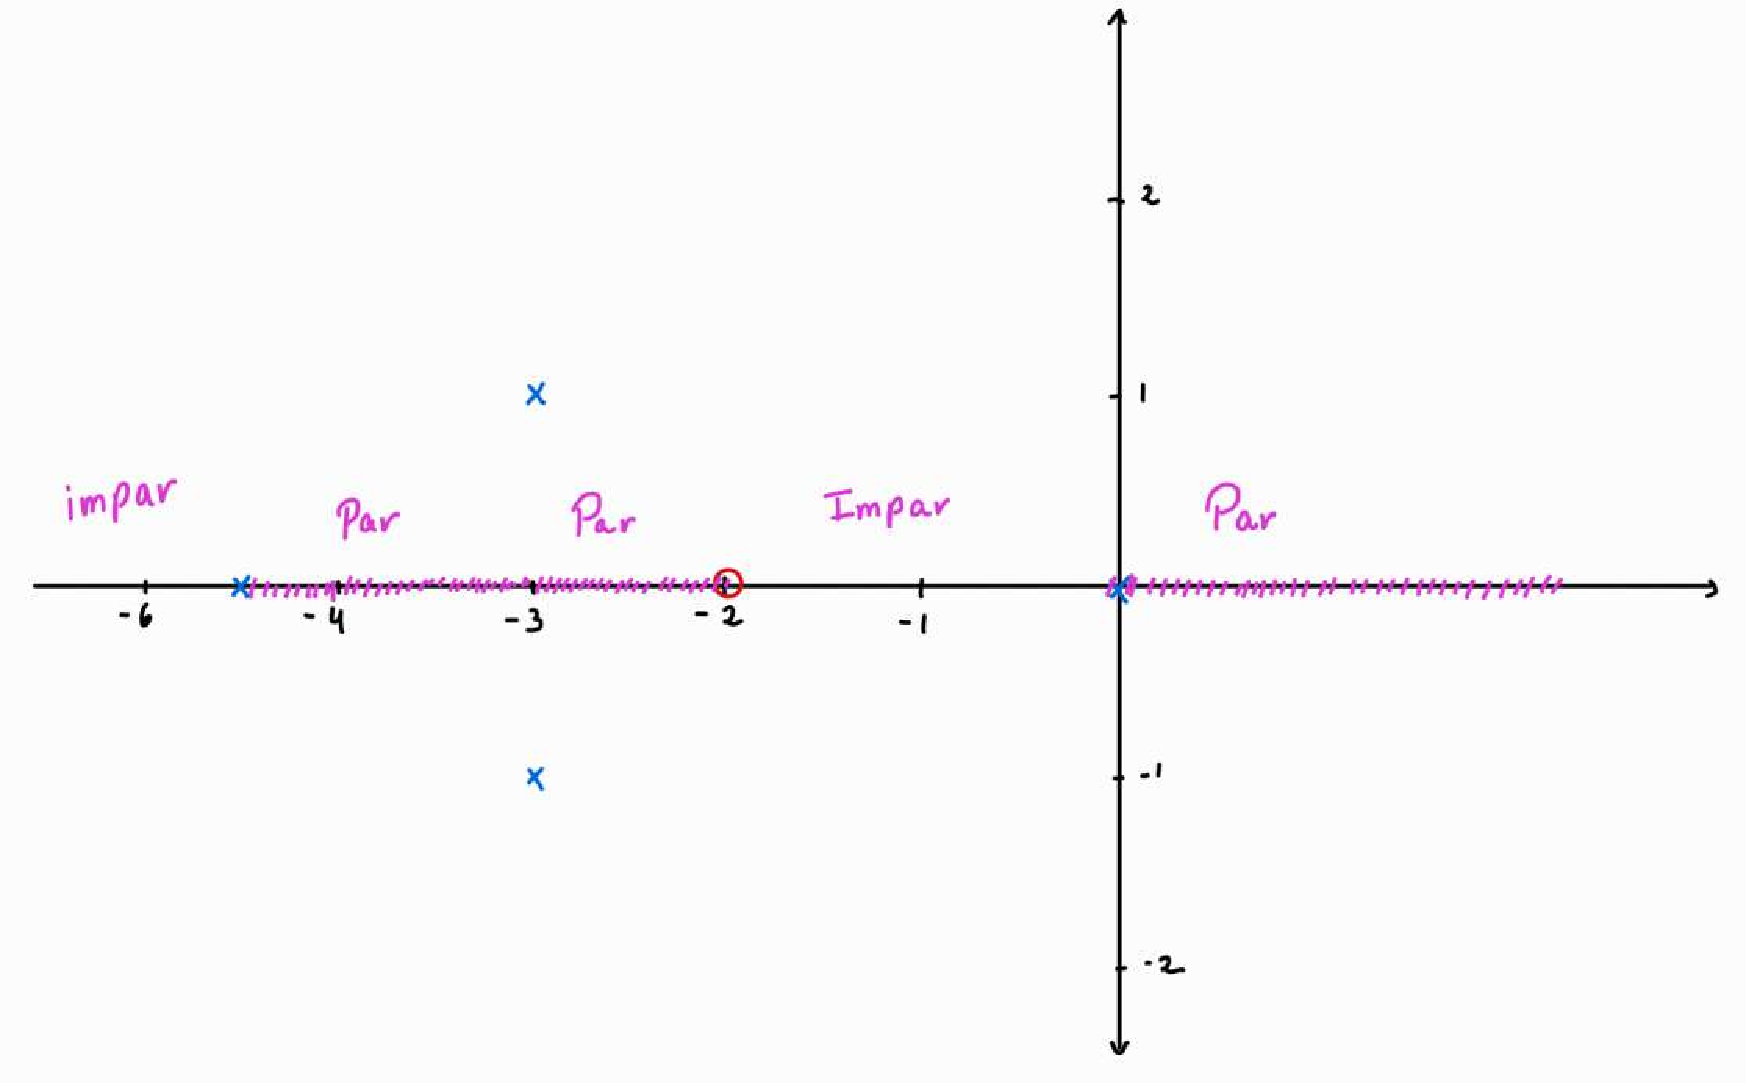
\includegraphics[width=0.7\textwidth]{Auxiliar_2_5}
  \caption{Esquema de la cuerda colgante con tensiones variables.}
  \label{fig:esquema-tension}
\end{figure}
De aquí se observa que, para $z_2>z_1$,
\begin{align}
  T(z_{2}) > T(z_{1}).
\end{align}
Así, cuanto más arriba, mayor tensión y, por tanto, mayor rapidez $c(z)$. El pulso que sube se propaga más rápido que el que baja y, en consecuencia, llega primero a su extremo (el superior).

\subsection*{Resolución 4.2}
Como el pulso que sube viaja más rápido, alcanza antes el techo (extremo fijo) y se refleja con inversión de fase; el pulso que baja llega después al extremo inferior (libre) y se refleja sin inversión. Cuando ambos regresan y se cruzan por primera vez, el pulso superior lleva ventaja temporal, por lo que
\boxed{\textbf{se encuentran por debajo del centro}}. Además, en ese instante tienen signos opuestos (uno invertido y el otro no), de modo que la superposición es \emph{destructiva} (se cancelan momentáneamente).
\end{solution}
%--------------------------
\question El túnel de una mina abandonada se proyecta hacia el interior de la montaña donde fue construido. Se quiere calcular el largo del túnel, pero es peligroso entrar en él. Entonces, usted decide tratar de establecer resonancias de \emph{onda estacionaria} en su interior. Usando un amplificador subsónico y un parlante encuentra resonancias a \(4.5\,\text{Hz}\) y \(6.3\,\text{Hz}\), y a ninguna otra frecuencia entre éstas. Además, se supone que la rapidez del sonido en el túnel es \(335\,\text{m/s}\) por estar a una temperatura inferior a la ambiente. A partir de sus medidas, estime la longitud del túnel \(L\). Justifique la elección de las condiciones de borde en los extremos del túnel.
%--------------------------
\begin{solution}

\subsection*{Resolución 5.1}
Dada el enunciado es posible modelar el túnel como un ducto \textit{abierto–cerrado} (boca abierta al aire y fondo rígido) y con largo L, con lo que tenemos que:
\begin{align}
  \lambda_{n}&= \frac{2l}{n}\\
  \lambda_{n+1} &= \frac{2l}{n+1}
\end{align}
Por otro lado tendremos que la velocidad del sonido sera igual para ambas frecuencias sonoras $f_n$ y $f_{n+1}$ por lo tanto:
\begin{align}
  v_{s} &= \lambda_{n}f_{n}\\
        &= \frac{2l}{n}f_{n}
\end{align}
Por otro lado tenemos que:
\begin{align}
  v_{s}&= \lambda_{n+1}f_{n+1}\\
       &= \frac{2l}{n+1}f_{n+1}
\end{align}
Luego podemos igualar ambas expresiones de velocidad:
\begin{align}
  \frac{2l}{n}f_{n} &= \frac{2l}{n+1}f_{n+1}\\
  \frac{f_{n}}{n} &= \frac{f_{n+1}}{n+1}\\
  f_{n}(n+1) &= f_{n+1}n\\
  f_{n} &= n(f_{n+1}-f_{n})\\
  n&= \frac{f_n}{f_{n+1}-f_n}
\end{align}
Luego tenemos que reemplazando esa expresion en la velocidad, tendremos que:
\begin{align}
  v_s = \frac{2l(f_{n+1}-f_n)}{f_n} \cdot f_n = 2l(f_{n+1}-f_n)\\
\end{align}
Con lo que despejando el valor de l tenemos que:
\begin{align}
  l= \frac{v_{s}}{2(f_{n+1}-f_n)}
\end{align}
Reemplazando los datos por enunciado tenemos que:
\begin{align}
  l= \frac{335}{2(6.3-4.5)}\;\text{m} = 93.1\;\text{m}
\end{align}
Con lo que se obtiene \(\boxed{93~\text{m}}\). correspondiente al largo del túnel.
\end{solution}
%--------------------------
\end{questions}
\end{document}